\documentclass[letter, 10pt]{article}
\usepackage[utf8]{inputenc}
\usepackage[spanish]{babel}
\usepackage{amsfonts}
\usepackage{amsmath}
\usepackage{caption}
\usepackage{multirow}

% \usepackage[dvips]{graphicx}
\usepackage{url}
\usepackage[top=3cm,bottom=3cm,left=3.5cm,right=3.5cm,footskip=1.5cm,headheight=1.5cm,headsep=.5cm,textheight=3cm]{geometry}
\usepackage[pdftex]{graphicx}
\usepackage{tikz}
\usetikzlibrary{calc,shapes.multipart,chains,arrows}
\usepackage{algorithm}
\usepackage{algpseudocode}

\tikzset{
    squarecross/.style={
        draw, rectangle,minimum size=18pt,
        inner sep=0pt, text=black,
        path picture = {
            \draw[black]
            (path picture bounding box.north west) --
            (path picture bounding box.south east)
            (path picture bounding box.south west) --
            (path picture bounding box.north east);
        }
    }
}
\begin{document}
\title{Inteligencia Artificial \\ \begin{Large}Informe Final: Problema Green Vehicle Routing Problem (GVRP)\end{Large}}
\author{Lucio Fondón Rebolledo}
\date{\today}
\maketitle

%--------------------No borrar esta secci\'on--------------------------------%
\section*{Evaluaci\'on}

\begin{tabular}{ll}
Mejoras 2da Entrega (10\%): &  \underline{\hspace{2cm}}\\
C\'odigo Fuente (10\%): &  \underline{\hspace{2cm}}\\
Representaci\'on (15\%):  & \underline{\hspace{2cm}} \\
Descripci\'on del algoritmo (20\%):  & \underline{\hspace{2cm}} \\
Experimentos (10\%):  & \underline{\hspace{2cm}} \\
Resultados (10\%):  & \underline{\hspace{2cm}} \\
Conclusiones (20\%): &  \underline{\hspace{2cm}}\\
Bibliograf\'ia (5\%): & \underline{\hspace{2cm}}\\
 &  \\
\textbf{Nota Final (100)}:   & \underline{\hspace{2cm}}
\end{tabular}
%---------------------------------------------------------------------------%
\vspace{2cm}


\begin{abstract}

En este trabajo se realizará un breve estudio del problema de optimización de Green Vehicle Routing Problem (GVRP), el cual consiste en minimizar la distancia recorrida por una flota de vehículos que deben realizar repartos a ciertos clientes predispuestos en posiciones fijas. Esta flota de vehículos debe iniciar su recorrido en un depósito y al finalizar deben volver a este. Durante su recorrido, los vehículos pueden detenerse a recargar combustible si es que éstos lo requieren. Se presentará un modelo matemático y sus respectivas técnicas utilizadas a lo largo de los años. Además, se presentarán, describirán e implementarán algoritmos basados en técnicas incompletas, utilizando una técnica Greedy y luego Simullated Annealing para la resolución del problema. Finalmente, se concluirá respecto a los puntos realizados en el documento.
% Resumen del informe en no m\'as de 10 l\'ineas, donde se sintetice el problema que se trata y sirva para que un lector no involucrado comprenda el objetivo del documento.
\end{abstract}

\section{Introducci\'on}

% Una explicaci\'on breve del contenido del informe, es decir, detalla: Prop\'osito, Estructura del Documento, Descripci\'on (muy breve) del Problema y Motivaci\'on.

Durante las últimas décadas, se ha dado cada vez más importancia al cuidado del medio ambiente en general, donde los gobiernos y empresas se han dedicado a tomar medidas para poder contaminar lo menos posible y atenerse a lo que son las \emph{políticas verdes}, ya que las logísticas que se utilizan hoy en día para la realización de ciertos procesos no son convenientes a largo plazo para el sostenimiento de la calidad del planeta ni el medio ambiente.
\\

Existen una gran cantidad de problemas que se atienen a lo que son las políticas verdes. Uno de los problemas que se estudiará será el de Green Vehicle Routing Problem (GVRP), con el fin de poder entender mejor como resolver esta clase de problemas y analizar la dificultad asociada a este. El GVRP consiste en minimizar la distancia recorrida por una flota de vehículos que deben realizar entregas a clientes, partiendo desde un depósito, para luego volver a éste. Durante el trayecto, pueden detenerse a recargar combustible, el cuál es un combustible alternativo que utilizan los vehículos, con el objetivo de minimizar el impacto ambiental producido por éstos. Esto puede parecer una tarea no muy difícil de realizar, pero la dificultad recae en el uso de combustible alternativo en los autos que se utilizarán en la flota, ya que, al ser combustible alternativo, también es menos común su uso, por lo que las estaciones de recarga de combustible serán más escasas.
\\

Primero, se definirá el problema de una manera más coloquial, señalando las principales características del problema, sus restricciones y objetivos, además de mostrar también las principales variantes que existen del problema. Luego, se realizará el \emph{Estado del Arte} del problema, en donde se hará hincapié principalmente en los métodos y algoritmos más utilizados para este tipo de problema, mostrando los distintos \emph{approach} que se han utilizado por investigadores para tratar de resolver este problema.
\\

Después, se presentará un modelo matemático para el problema en cuestión, con el fin de poder acercarse al problema y a su solución desde una perspectiva más matemática y computable, analizando más en profundidad las partes que componen al problema, tales como las variables, su función objetivo, sus restricciones y parámetros.
\\

Luego, se detallará la representación de las soluciones del problema, indicando la forma en que se representarán las soluciones de las instancias predispuestas para el problema. También, se detallará la descripción de los algoritmos de Greedy y Simullated Annealing para poder implementar la resolución del problema.
\\

Además, se presentarán las respectivas experimentaciones con las instancias dadas para la resolución del problema, para luego mostrar los resultados obtenidos de estas experimentaciones.
\\

Finalmente, se mostrarán conclusiones con respecto a todo lo lo presentado anteriormente, especialmente respecto a ventajas y desventajas de utilizar o no ciertas técnicas para abordar el problema.


\section{Definici\'on del Problema}
\label{definicion}
Uno de los problemas combinatoriales de optimización más famosos y estudiados es el Vehicle Routing Problem (VRP), el cual consiste en minimizar la distancia recorrida de una flota de vehículos que deben realizar entregas a un conjunto de clientes, con el objetivo de abaratar costos durante el trayecto. Los VRP caen en la clasificación de ser un problema \emph{NP-Hard}, dado que es una generalización del TSP \cite{RePEc:inm:ormnsc:v:6:y:1959:i:1:p:80-91}. Antes de presentar las variantes del GVRP, se nombrarán y describirán brevemente las variantes más importantes que surgen del VRP, dado que están relacionadas también con las variantes de GVRP:
\\

% LO QUE SIGUE VA EN EL ESTADO DEL ARTE
% Mirando desde una perspectiva histórica, el VRP surge a finales de los 50 con los estudios realizados por Dantzig y Ramser \cite{LIN20141118}, en donde ellos indican que el VRP es una generalización del Traveling Salesman Problem (TSP) si es que se le agregan ciertas restricciones a considerar en el contexto del problema del VRP \cite{RePEc:inm:ormnsc:v:6:y:1959:i:1:p:80-91}. Lo anterior es considerado un hincapié inicial para las tantas otras variantes que surgen del problema, hasta finalmente llegar a la variante del GVRP. Ahora, se nombrarán y describirán brevemente las variantes más importantes que surgen de las ideas de Dantzig y Ramser:
\begin{itemize}
    \item \textbf{\emph{Time-dependent VRP}} (TDVRP - 1966): Los primeros trabajos que consideraron esta variante del problema recae en los estudios realizados por Cooke y Halsey. La principal diferencia con VRP es que la distancia entre los puntos a repartir (ya sean clientes, estaciones de  servicio o el depósito) varía dependiendo en qué momento del día se encuentre, ya sea por ejemplo, por condiciones climáticas, horas punta de tráfico, etc. La introducción del TDVRP fue muy relevante para estudios posteriores, en especial los problemas de optimización de redes de tráfico reales  \cite{Cooke1966TheSR}.

    \item \textbf{\emph{Multi-depot VRP}} (MDVRP - 1969): Primeramente estudiado por Tillman en 1969, esta variante contempla que, en vez de que exista un sólo depósito inicial de donde salgan y tengan que volver los vehículos, existan múltiples depósitos de éstos. Este problema se origina principalmente debido a problemas de distribucion de la vida real tales como el reparto de comidas, productos químicos, reparto de productos de una empresa, etc. \cite{doi:10.1287/trsc.3.3.192}
    
    % \item \textbf{\emph{Periodic VRP}} (PVRP - 1974): En esta variante, se considera, además de las restricciones ya mencionadas anteriormente del VRP original, que los clientes deben ser visitados en diferentes días dentro de la semana, por lo que el objetivo principal de esta variante es minimizar el costo total de la ruta a lo largo de la planificación de la semana. Beltrami y Bodin en 1974 propusieron algoritmos considerando lo anterior \cite{https://doi.org/10.1002/net.3230040106}.
    
    \item \textbf{\emph{Dynamic VRP}} (DVRP - 1976): En las variantes anteriores, se lidia con información previa acerca de cómo y a donde se deben realizar las entregas, sin embargo, en la vida real no siempre es así. Speidel (1976) y Psaraftis (1980) estudiaron el problema de manera en que la información se va recibiendo en tiempo real, tales como localización de los vehículos y los pedidos de los clientes. Ejemplos de esto son lo servicios de emergencia, servicios de rescate, etc.  \cite{Speidel1976EDPASSISTEDFS} \cite{doi:10.1287/trsc.14.2.130}.
    
    \item \textbf{\emph{VRP with Time windows}} (VRPTW - 1977): Hasta ahora, no se han considerado los tiempos de servicio que se deban cumplir como restricciones. Russell (1977) presentó una heurística para este caso y propuso dos tipos de time windows \cite{doi:10.1287/opre.25.3.517}:
    \begin{itemize}
        \item \emph{Hard Time Windows}: El vehículo debe llegar antes o justo después del tiempo de entrega especificado, y no se permite llegar tarde. Además, si llega antes, el vehículo debe esperar hasta que pase la ventana de tiempo.
        \item \emph{Soft Time Windows}: Las violaciones a las ventanas de tiempo se permiten pero se penalizan a un cierto costo.
    \end{itemize}
\end{itemize}
\\

Teniendo lo anterior en cuenta, se da paso al GVRP (2012) \cite{ERDOGANMILLERHOOKS}. Debido al constante deterioro del medioambiente en el planeta, los gobiernos y empresas comenzaron a adoptar las llamadas logísticas verdes dentro de sus operaciones, es por esto que nace el problema que estudiaremos acá, el Green Vehicle Routing Problem (GVRP), el cual es una variante del VRP en donde los vehículos predispuestos para realizar las entregas a los clientes utilizan un combustible alternativo, con el fin de dejar la menor cantidad de contaminación posible en la realización de sus tareas.
\\

El GVRP consiste en realizar una ruta de entregas de una cierta flota de vehículos que parten desde un mismo depósito hacia un conjunto de clientes que se encuentran dispersos geográficamente en un área en particular, para luego volver al mismo depósito inicial, esto con el fin de poder minimizar la distancia recorrida por esta flota de vehículos y así poder también abaratar los costos asociados al trayecto en general. Estos vehículos pueden realizar paradas en caso de que requieran combustible. Notar que, al utilizar combustible alternativo por ser GVRP, las estaciones serán más limitadas. Además, debido a que GVRP es una variante de VRP, es considerado también un problema \emph{NP-Hard}. Ahora, se presentarán variantes que han salido del GVRP en los últimos años:\\
\begin{itemize}
    \item \textbf{\emph{Fuzzy GVRP}} (F-GVRP - 2018): F-GVRP fue propuesto por primera vez por los autores Poonthalir y Nadarajan \cite{FGVRP}. Las principales diferencias con GVRP recaen en que F-GVRP es multiobjetivo, ya que busca minimizar el costo de la ruta asociada y además el consumo de combustible, GVRP solo minimiza el costo de la ruta. Además, en GVRP, la velocidad y el consumo de combustible es constante, en F-GVRP no lo son.

    \item \textbf{\emph{Capacitated GVRP}} (CGVRP - 2018): CGVRP fue introducido por Zhang \cite{CGVRP}. La diferencia de esta variante con la original de GVRP recae principalmente en que considera restricciones que están asociadas a las capacidades de almacenamiento de inventario que puedan llevar los autos pertenecientes a la flota.
    
    \item \textbf{\emph{Pollution routing problem}} (PRP - 2011): Introducida por primera vez por Bektas y Laporte \cite{PRP}. Esta variante del GVRP se diferencia debido a que la función objetivo se concentra en minimizar el gasto de combustible de los autos y el costo de los conductores. 
    
    \item \textbf{\emph{Energy-minimizing vehicle routing problem}} (EMVRP - 2007): Presentado e investigado inicialmente por Kara et al. \cite{EMVRP}. En esta variante, su función objetivo se enfoca principalmente en minimizar el trabajo (o energía) producida por los vehículos, basándose en un función de costos que se obtiene a partir de los pesos de los vehículos de la flota y las distancias recorridas.

\end{itemize}
\\

Las principales variables a tener en cuenta dentro de este problema serán variables relacionadas a si cierto vehículo viaja de un punto a otro y variables relacionadas al tiempo de llegada de un vehículo a un punto y el combustible disponible en los vehículos. Además, se tienen que considerar ciertas restricciones que existen en el problema. Los vehículos están restringidos por una cantidad de distancia que pueden recorrer con la cantidad de combustible que almacenan. También, las visitas a un cliente tienen un tiempo de servicio asociado. Cuando un vehículo requiera llenarse de combustible, también tomará un tiempo de recarga de combustible. Además, los vehículos están restringidos a un tiempo de servicio que no pueden sobrepasar antes de volver al depósito. Por otro lado, cada cliente debe visitarse una sola vez por un solo vehículo. Por último, se tomará en consideración que no existe un límite de vehículos disponibles en la flota y que la velocidad de estos es constante.

% Explicaci\'on del problema que se va a estudiar, en qu\'e consiste, cu\'ales son sus variables , restricciones y objetivo(s) de manera general (en palabras, no una formulaci\'on matem\'atica). Debe entenderse claramente el problema y qu\'e busca resolver.
% Explicar si existen problemas relacionados.
% Destacar, si existen, las variantes m\'as conocidas.\\
% Redactar en tercera persona, sin faltas de ortograf\'ia y referenciar correctamente sus fuentes mediante el comando  \verb+\cite{ }+. Por ejemplo, para hacer referencia al art\'iculo de algoritmos h\'ibridos para problemas de satisfacci\'on 
%  de restricciones~\cite{MOGHDANI2021123691}.

\section{Estado del Arte}
\label{estado}
Como se mencionó anteriormente, el GVRP es una variante del problema original VRP. El Vehicle Routing Problem fue introducido por primera ver por Dantzig y Ramser (1959), y mencionan que el problema viene directamente del conocido Traveling Salesman Problem (TSP) \cite{RePEc:inm:ormnsc:v:6:y:1959:i:1:p:80-91}. El problema lo describen como un \emph{routing problem}, en donde camiones con gasolina debían repartir a ciertas estaciones de servicio geográficamente esparcidas en un espacio en particular. Propusieron un algoritmo basado en programación lineal entera, para poder obtener una solución cercana a la óptima. A esta variante inicial de VRP se le llamó \emph{Capacitated VRP} \cite{LIN20141118}.
\\

Lo anterior es considerado un hincapié inicial para las tantas otras variantes que surgen del problema, hasta finalmente llegar a la variante del GVRP. 
Se muestran a continuación los métodos y algoritmos utilizados en general para la resolución de los GVRP.\\

\begin{figure}[h]
    \centering
    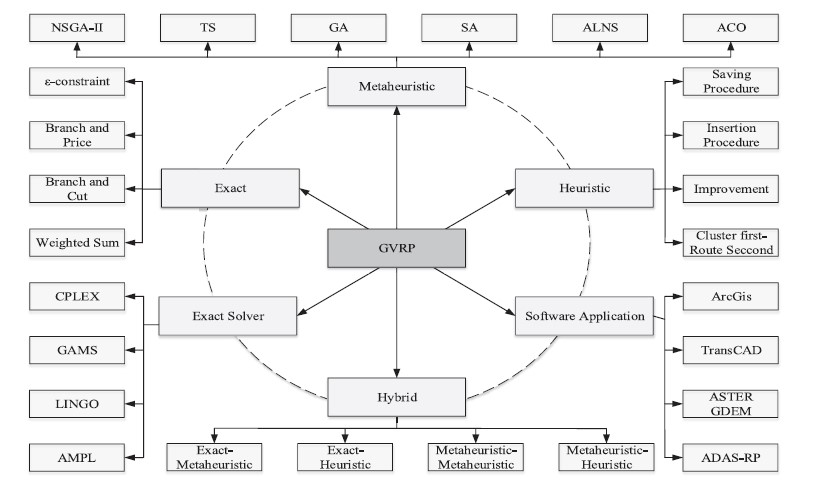
\includegraphics[width=12cm]{Algoritmos GVRP.jpg}
    \caption{Métodos de resolución más utilizados para GVRP  \cite{SYSTEMATICLITERATURE}}
    \label{fig:figura1}
\end{figure}

Se detallarán ahora brevemente algunos de los métodos utilizados más importantes para la resolución del GVRP:

\subsection{Algoritmos Exactos}
Dentro de los algoritmos exactos utilizados para poder resolver problemas de GVRP, podemos destacar:
\begin{itemize}
    \item \textbf{\emph{Programación Lineal Entera}}: Es sabido que la programación lineal entera ha sido uno de los primeros métodos en general para la resolución de problemas en donde se debían minimizar o maximizar una cierta variable para algún problema. En el caso de los problemas de GVRP no es distinto; Erdoğan y Miller-Hooks, quienes fueron las primeras autoras en proponer los GVRP como tal, propusieron el GVRP con un modelo de programación lineal entera mixta \cite{ERDOGANMILLERHOOKS}. Lo proponen también Andelmin y Bartolini, donde formulan la resolución con un método de programación lineal entera mixta con \emph{set partitioning} \cite{EXACTALGORITHM}. Por lo general, utilizan la modelación del problema como un programación lineal entera mixta y luego buscan distintos approach para resolver las instancias. Por ejemplo, en \cite{BRUGLIERI2019109} se modela el problema como programación lineal entera mixta, pero se resuelve utilizando un approach basado en caminos. Por otra parte, también se han utilizado técnicas de \emph{Branch and Price} \cite{BRANCHANDPRICE} y \emph{Branch and Cut} \cite{CHENG201797}. Sin embargo, las soluciones utilizando programación lineal entera, por lo general, no pueden escalar a problemas dentro de la vida real, específicamente por la gran cantidad de variables binarias que se generan, por lo que se hace muy difícil computacionalmente llegar a soluciones exactas óptimas \cite{LAPORTE1992345}.

\end{itemize}

\subsection{Algoritmos Aproximados}
En los algoritmos aproximados que se han utilizado a lo largo de la historia para resolver instancias del GVRP y sus variantes, podemos dividirlos en dos categorías: las \emph{heurísticas clásicas} y las \emph{metaheurísticas}. Dentro de las heurísticas clásicas se pueden destacar los siguientes métodos utilizados:

\begin{itemize}
    \item \textbf{\emph{Algoritmos de Ahorro}}: Clarke y Wrigth (1964) propusieron una heurística clásica para el VRP, y probablemente sea la más conocida para este tipo de problema, y generalmente se utiliza cuando el número de vehículos son una variable de decisión. Este método produjo soluciones cuyos valores se encuentran un $6.71\%$ por sobre las que se conocen \cite{CLASSICHEURISTICS}. En el contexto más contemporáneo con el problema del GVRP, se propuso en 2012 una utilización del método de Clarke y Wrigth modificado, logrando una optimización del $14.9\%$ en distancia recorrida \cite{ARANDAUSON}.
    
    \item \textbf{\emph{Algoritmos de Clustering}}: También, se han utilizado técnicas de agrupamientos de datos o \emph{clustering} para poder resolver instancias del GVRP. Si bien Erdoğan y Miller-Hooks proponen el modelo para resolver el problema como uno de programación lineal entera mixta, utilizan una heurística \emph{Density-Based Clustering Algorithm} (DBCA). Esta técnica aprovecha características que otras técnicas no consideran, tales como las propiedades espaciales del GVRP. La idea principal del algoritmo es tratar de agrupar en un círculo de radio $\epsilon$ una cantidad mínima de clientes junto con las estaciones de recarga ($minPts$). Cada clúster representará una ruta factible que un vehículo de la flota puede recorrer. Este algoritmo es comparado con un algoritmo de ahorro de Clake y Wright modificado, en donde se concluye que DBCA tiende a tener resultados un poco más óptimos \cite{ERDOGANMILLERHOOKS}.
    

\end{itemize}
Por otro lado, dentro de las metaheurísticas, se pueden dividir en dos ramas:
\begin{itemize}
    \item \textbf{\emph{Técnicas de Búsqueda Local}}: Estas técnicas se basan en explotar el espacio de soluciones al moverse iterativamente desde una solución a otra más prometedora dentro de su vecindario \cite{LIN20141118}. Dentro del GVRP, está \emph{Tabu Search} (TS), que Ehmke lo utiliza en sus estudios para modelar una resolución al problema de GVRP principalmente porque, para las variantes de VRP, Tabu Search ha dado buenos resultados \cite{EHMKE}. También se ha utilizado \emph{Simulated Annealing} (SA) en varias ocasiones \cite{SALOCAL}, utilizándose también en algoritmos híbridos de SA con branch and cut  (B\&C), para poder diversificiar e intensificar de manera correcta en el espacio de búsqueda de soluciones \cite{BYCSA}.
    
    \item \textbf{\emph{Técnicas basadas en Población}}: Los métodos basados en población mantienen un \emph{pool} de soluciones prometedoras, y se actualiza este pool a medida que encuentra otras mejores. En esta categoría se encuentran los \emph{Genetic Algorithms} (GA) y los \emph{Ant Colony Optimization} (ACO). En el caso de los GA, se ha demostrado que se obtiene un $17.91\%$ de mejora en la solución que si se utilizan técnicas de modelado de TSP para resolver el problema de GVRP \cite{GENETIC}. Para los ACO, se demuestra que para instancias de gran tamaño, tienen muy buenos resultados, por lo que utilizar ACO es útil para poder resolver instancias del mundo real de GVRP.\cite{ACO}.   
\end{itemize}

Las publicaciones en los últimos años acerca de resoluciones y métodos nuevos para el GVRP y variantes del VRP siguen creciendo. Sin embargo, los estudios que existen de las variantes de GVRP son, limitados principalmente debido a que involucra muchos factores que son complicados hoy en día, tales como energía e impacto ambiental, polución, planificamiento urbano, etc \cite{SYSTEMATICLITERATURE}.
\\

En general, los problemas de GVRP que se analizan hoy en día tienen que ver con aquellos que tienen comportamiento \emph{no determinista}, es decir, \textbf{GVRP con incertidumbres}. Algunos ejemplos son los GVRP \emph{fuzzy chance-constrained mixed integer non-linear programming model} \cite{Sun2018ATF} y los de optimización estocástica \cite{RAHIMI201759}. 

% La informaci\'on que describen en este punto se basa en los estudios realizados con antelaci\'on respecto al tema.
% Lo m\'as importante que se ha hecho hasta ahora con relaci\'on al problema. Deber\'ia responder preguntas como las siguientes:
% ?`cu\'ando surge?, ?`qu\'e m\'etodos se han usado para resolverlo?, ?`cu\'ales son los mejores algoritmos que se han creado hasta
% la fecha?, ?`qu\'e representaciones han tenido los mejores resultados?, ?`cu\'al es la tendencia actual para resolver el problema?, tipos de movimientos, heur\'isticas, m\'etodos completos, tendencias, etc... Puede incluir gr\'aficos comparativos o explicativos.\\



\section{Modelo Matem\'atico}
\label{modelo}
Ahora, se presentará un modelo matemático para el problema del GVRP, el cuál se define como un grafo completo no dirigido $G = (V,E)$. En este caso, se utilizará el modelo planteado por Erdoğan y Miller-Hooks \cite{ERDOGANMILLERHOOKS}. Este estudio fue el primero en introducir lo que son los \emph{Alternative Fuel-powered Vehicles} (AFV) en el problema del GVRP, por lo que toma en cuenta lo que necesitamos para poder resolver el problema utilizando políticas verdes y obtener una solución óptima en minimización de distancia recorrida y costos de entrega. Cabe destacar que este modelo es formulado en base a programación lineal entera mixta.

\subsection{Parámetros}
\begin{itemize}
    \item $I$: Conjunto de vértices de los clientes.
    \item $F$: Conjunto de vértices de las estaciones de recarga.
    \item $v_0$: Depósito inicial (punto de partida y llegada de los vehículos).
    \item $V$: Conjunto de todos los vértices (Notar que $V = \{v_0\} \cup I \cup F$).
    \item $d_{ij}$: Distancia desde el vértice $i$ hasta el vértice $j$.
    \item $p_i$: Tiempo de servicio que toma en el vértice $i$ (Si $i \in I$, entonces corresponde al tiempo de servicio al cliente. Si $i \in F$, entonces corresponde al tiempo de recarga de combustible en una estación).
    \item $Q$: Capacidad del tanque de combustible del vehículo.  (El valor del combustible restante de un vehículo toma el valor de $Q$ cada vez que se recargue combustible).
    \item $r$: Velocidad de consumo de combutible del vehículo.
    \item $T_{max}$: Tiempo máximo de servicio del vehículo.
\end{itemize}

\subsection{Variables}
\begin{itemize}
    \item     $x_{ij} = \left\{
        \begin{array}{ll}
            1 & \quad \text{Si el vehículo viaja desde el vértice $i$ hasta el vértice $j$} \\
            0 & \quad \text{Caso contrario}
        \end{array}
    \right.$
    \item $y_j$ = Nivel de combustible del vehículo restante al llegar al vértice $j$.
    \item $\tau_j$ = Tiempo de arribo de un vehículo al vértice $j$. Se inicializa en $0$ partiendo desde $v_0$.
\end{itemize}

\subsection{Función objetivo}
\begin{align}
    \min F:
    & \sum_{\substack{(i,j)\in V\\ i \neq j}} d_{ij} x_{ij}
\end{align}
\begin{center}
    Ecuación 1: Función objetivo asociada al problema del GVRP propuesta por Erdoğan y Miller-Hooks. Busca minimizar la distancia total recorrida por un vehículo de la flota.
\end{center}

\subsection{Restricciones}
\begin{align}
    \sum_{\substack{j\in V\\ j \neq i}} x_{ij} = 1, & \quad \forall i \in I
\end{align}

\begin{center}
    Ecuación 2: Maneja que cada vértice perteneciente al conjunto de los clientes tenga un solo sucesor, ya sea una estación de recarga, otro cliente o el depósito inicial $v_0$.
\end{center}

\begin{align}
    \sum_{\substack{j\in V\\ j \neq i}} x_{ij} \leq 1, & \quad \forall i \in F
\end{align}

\begin{center}
    Ecuación 3: Se asegura que cada vértice perteneciente al conjunto de las estaciones de recarga tenga a lo más un sucesor, ya sea una estación de recarga, otro cliente o el depósito inicial $v_0$.
\end{center}

\begin{align}
    \sum_{\substack{i\in V\\ j \neq i}} x_{ji} - \sum_{\substack{i\in V\\ j \neq i}} x_{ij} = 0, & \quad \forall j \in V
\end{align}

\begin{center}
    Ecuación 4: Esta restricción se asegura que el número de llegadas a cada vértice perteneciente a $V$ sea el mismo que el número de salidas.
\end{center}


% \begin{align}
%     \sum_{\substack{j\in V \text{\textbackslash} \{0\}}} x_{0j} \leq m
% \end{align}

% \begin{align}
%     \sum_{\substack{j\in V \text{\textbackslash} \{0\}}} x_{j0} \leq m
% \end{align}

\begin{align}
    \tau_j \geq \tau_i + (t_{ij} - p_j)x_{ij} - T_{\text{max}}(1 - x_{ij}), & \quad \forall i \in V, \forall j \in V \text{\textbackslash}\{0\}, i \neq j
\end{align}

\begin{center}
    Ecuación 5: Esta restricción es necesaria para tener registro del tiempo en el que cada vértice $i$ es visitado y el tiempo en que le toma llegar al vértice $j$, para así poder prevenir subrutas.
\end{center}


\begin{align}
    0 \leq \tau_0 \leq T_{\text{max}}
\end{align}

\begin{center}
    Ecuación 6: Se asegura de que cada vehículo no exceda el tiempo máximo $T_{\text{max}}$ de tiempo de llegada de vuelta al depósito, especificando el tiempo con el que parte el vehículo desde el depósito $v_0$.
\end{center}

\begin{align}
    t_{0j} \leq \tau_j \leq T_{\text{max}} - (t_{j0} + p_j), \quad \forall j \in V \text{\textbackslash}\{0\}
\end{align}

\begin{center}
    Ecuación 7: Se asegura que cada vehículo termine la ruta en el tiempo máximo $T_{\text{max}}$.
\end{center}

\begin{align}
    y_j \leq y_i - r \cdot d_{ij}x_{ij} + Q(1 - x_{ij}), \quad \forall j \in I \text{ y } i \in V, i \neq j
\end{align}

\begin{center}
    Ecuación 8: Se encarga de reducir el nivel de carga de combustible del vehículo que llega a un vértice $j$, considerando la distancia recorrida desde $i$ hasta $j$ y la velocidad $r$ a la que va el vehículo.
\end{center}

\begin{align}
    y_j = Q, & \quad \forall j \in F
\end{align}

\begin{center}
    Ecuación 9: Encargada de setear nuevamente el nivel de combustble de un vehículo al visitar a una estación de recarga.
\end{center}

\begin{align}
    y_j \geq \min \{r \cdot d_{j0}, r(d_{jl} + d_{l0})\}
\end{align}

\begin{center}
    Ecuación 10: Garantiza que el vehículo cuente con el combustible necesario para poder volver al depósito o a una estación de recarga.
\end{center}

\subsection{Naturaleza de las Variables}
\begin{itemize}
    \item $x_{ij}$: Variable de decisión booleana. $x \in \{0,1\}$
    \item $\tau_j, y_j$: Variables tipo entero. $\tau_j, y_j \in \mathbb{Z}$
\end{itemize}


% Uno o m\'as modelos matem\'aticos para el problema, idealmente indicando el espacio de b\'usqueda para cada uno. Cada modelo debe estar correctamente referenciado, adem\'as no debe ser una imagen extraida. Tambi\'en deben explicarse en detalle cada una de las partes, mostrando claramente la funci\'on a maximizar/minimizar, variables y restricciones. Tanto las f\'ormulas como las explicaciones deben ser consistentes.
\newpage

\section{Representación}

Para efectos de este documento, la representación de la solución escogida viene dada por una lista enlazada simple, en donde esta lista estará compuesta de nodos secuencialmente unidos por un puntero. Estos nodos tendrán como dato (e identificación) al nodo que se visita durante la ruta. Una representación posible de una solución podría ser:\\

\begin{tikzpicture}[
        list/.style={
            very thick, rectangle split,
            rectangle split parts=2, draw,
            rectangle split horizontal, minimum size=18pt,
            inner sep=3pt, text=black,
            %rectangle split part fill={red!20, blue!20}
        },
        ->, start chain, very thick
      ]

    \node[list,on chain] (A) {\texttt{d0}};
    \node[list,on chain] (B) {\texttt{c7}};
    \node[list,on chain] (C) {\texttt{c4}};
    \node[list,on chain] (D) {\texttt{c9}};
    \node[list,on chain] (E) {\texttt{f1}};
    \node[list,on chain] (F) {\texttt{c1}};
    \node[list,on chain] (G) {\texttt{d0}};
    \node[squarecross]   (H) [right=of G] {};
    \draw[*->] let \p1 = (A.two), \p2 = (A.center) in (\x1,\y2) -- (B);
    \draw[*->] let \p1 = (B.two), \p2 = (B.center) in (\x1,\y2) -- (C);
    \draw[*->] let \p1 = (C.two), \p2 = (C.center) in (\x1,\y2) -- (D);
    \draw[*->] let \p1 = (D.two), \p2 = (D.center) in (\x1,\y2) -- (E);
    \draw[*->] let \p1 = (E.two), \p2 = (E.center) in (\x1,\y2) -- (F);
    \draw[*->] let \p1 = (F.two), \p2 = (F.center) in (\x1,\y2) -- (G);
    \draw[*->] let \p1 = (G.two), \p2 = (G.center) in (\x1,\y2) -- (H);

\end{tikzpicture}
\\


La anterior solución a una instancia fictica del problema representa una ruta posible que puede tomar un vehículo en cuestión, es decir, el vehículo parte desde el depósito \texttt{d0}, para luego ir a visitar a 3 clientes, \texttt{c7-c4-c9}. Despúes va a visitar una estación de recarga \texttt{f1}, para luego visitar a un cliente más \texttt{c1}, y se devuelve al depósito \texttt{d0}.
\\

Esta representación fue elegida más que nada por su fácil uso y secuencialidad intrínseca que conlleva, dado que es fácil observar cual es claramente la ruta que lleva un vehículo asociado a la flota. También, implementar esta representación no es difícil, ya que solo se tienen que representar los nodos correspondientes a cada tipo de punto de llegada o salida (ya sea depósito, estación o cliente a visitar) y conectarlos mediante un puntero, así hasta llegar al último nodo, que se conectará a un nodo nulo para poder representar que se llegó al final y se acabó el recorrido del vehículo.
\\

En cuanto a la relación que tiene esta representación con el espacio de búsqueda asociado al problema de GVRP, esta no reduce el espacio de búsqueda en sí, ya que el espacio de búsqueda asociado consistiría en obtener todos los subconjuntos posibles de rutas que se puedan obtener a partir de una instancia provista para el problema, los cuales representarían las soluciones factibles e infactibles del problema, pero al fin y al cabo estas soluciones si podrían ser reproducidas por esta representación elegida. Por otra parte, el espacio de búsqueda en sí se ve reducido más por la utilización del algoritmo Greedy que se detallará más adelante, ya que solo obtendrán soluciones factibles del problema.

% Para efectos de este documento, la representación de la solución de una instancia del problema del GVRP estará dada por un arreglo de \texttt{chars} (o en su defecto, \texttt{strings}), es decir, una cadena de carácteres, en donde se mostrarán el recorrido nodo a nodo que tuvo que realizar uno de los vehículos de la flota. Por ejemplo, una solución para una instancia ficticia del problema podría ser la siguiente:\\

% \noindent\texttt{Millas recorridas: 450}\\
% \texttt{Clientes atendidos: 7}\\
% \texttt{Vehículos: 2}\\
% \texttt{Tiempo de ejecución: 0.024}\\
% \\
% \texttt{d0-c7-c4-c9-f1-c1-d0 200   608   0}\\
% \texttt{d0-c2-c5-f2-c2-d0 250   502   0}\\

% En donde las primeras 4 líneas del output de la solución serán la distancia en millas recorridas en total por los vehículos de la flota, la cantidad de clientes atendidos en la solución de la instancia, los vehículos utilizados y el tiempo de ejecución del algoritmo. Luego, se muestran los recorridos realizados por cada vehículo participante en la solución de la instancia del problema, en donde se puede ver que el recorrido de los nodos está separado por un guión (\texttt{-}), partiendo desde el nodo inicial \texttt{d0} y volviendo a este. Además, se puede ver que en los outputs de los recorridos de los vehículos hay 3 enteros que le siguen; el primero es la distancia recorrida por el vehículo en millas, lo sigue el tiempo que le tomó realizar el recorrido y por último la distancia excedida.

\newpage

\section{Descripción del algoritmo}

El algoritmo que se utilizará en este documento será una mezcla de tipo \emph{Greedy}, para poder obtener una solución factible inicial, y luego a esta solución mejorarla utilizando un approach algorítmico con \emph{Simullated Annealing}.\\

El algoritmo greedy funcionará de la siguiente forma: se partirá desde un nodo inicial (depósito) \texttt{d0}, que se nombrará como \texttt{nodoActual}. Luego, se realizará una visita de nodos utilizando la distancia mínima que haya desde el nodo actual \texttt{d0} hasta el nodo a visitar (es decir, la función  miope a utilizar en el problema sería escoger el nodo de distancia mínima desde el nodo actual al nodo a visitar y la función de evaluación la distancia total recorrida por los vehículos), llámese \texttt{nodoVisitado}. Si ese nodo no ha sido visitado y esa distancia no hace que se agote el combustible, entonces se visitará el nodo y se actualizará \texttt{nodoActual} a \texttt{nodoVisitado}. En caso contrario, se escogerá el siguiente nodo no visitado con la distancia mínima del nodo actual al nodo visitado, y así hasta que encuentre uno factible. El algoritmo tendrá como tope de término que el tiempo máximo de servicio del vehículo no se exceda. Un nodo factible a visitar se denotará como que no exceda el combustible ni el tiempo al visitarlo y para volver al depósito, entonces se asegurará si o si de tener tiempo siempre para volver al depósito. Esta factibilidad se manejará en la posterior implementación.

\begin{algorithm}
\caption{GreedyGVRP(C[1\ldots $\#Customers$], F[1\ldots $\#Stations$], MaxTime, MaxDistance, Speed,  ServiceTime, RefuelTime)}\label{alg:cap}
    \begin{algorithmic}
        \State $S \gets \emptyset$
        \State $nodoActual \gets d_0$
        \State $actualTime \gets 0$
        \State $actualDistance \gets 0$
        \State $actualEstanque \gets MaxDistance$
        \State $Flag \gets TRUE$
        \While{$Flag$}
            \State $nodoVisitado \gets \text{select a minimum distance feasible node from array C}$
            \State $distance \gets haversineDistance(\text{nodoActual, nodoVisitado})$
            \If{$actualEstanque - distance < 0$}
                \State $estacionVisitada \gets \text{select a minimum distance feasible node from array F}$
                \State $distance \gets haversineDistance(\text{nodoActual, estacionVisitada})$
                \State $actualDistance \gets actualDistance + distance$
                \State $actualEstanque \gets MaxDistance$
                \State $actualTime \gets actualTime + RefuelTime$
                \State $S \gets S \cup \{estacionVisitada\}$
            \Else
                \State $actualDistance \gets actualDistance + distance$
                \State $actualEstanque \gets actualEstanque - distance$
                \State $actualTime \gets actualTime + ServiceTime$
            \EndIf
            
            \State $tripTime \gets actualDistance/Speed$
            \State $actualTime \gets actualTime + tripTime$

            
            \If{$actualTime > MaxTime$}
                \State $Flag \gets FALSE$
            \Else
                \State $S \gets S \cup \{nodoVisitado\}$
            \EndIf
        \EndWhile
    \end{algorithmic}
\end{algorithm}

\newpage
Ahora, se presentará un algoritmo de SA para tratar de mejorar la solución entregada por el algoritmo greedy presentado anteriormente. Este algoritmo de SA funciona muy parecido a los algoritmos de SA por definición, los cuales \emph{intensifican} al realizar un búsqueda local en el vecindario de la solución provista por el algoritmo greedy y \emph{diversifica} al utilizar las técnicas de enfriamiento de la temperatura, para poder aceptar soluciones de mejor calidad. Es decir, se irán revisando los vecinos de la solución actual mediante movimientos, para luego enfriar la temperatura, para así haber menos probabilidades de aceptar una solución de peor calidad. Solo se deben definir correctamente los criterios de término y los movimientos para cambiar la solución actual. Para efectos de esta implementación, se utilizará como movimiento un intercambio entre las visitas que se hacen a los nodos que estén consecutivos. Para evidenciar un ejemplo, se usará el caso ficticio que se mostró anteriormente en la representación de las soluciones:\\

\texttt{d0-c7-c4-c9-f1-c1-d0}\\

Entonces, en este caso, se pueden realizar 4 posibles intercambios entre el orden de visita de los nodos: \texttt{c7-c4}, \texttt{c4-c9}, \texttt{c9-f1} y \texttt{f1-c1}. Claramente, al ser una instancia ficticia del problema, se está asumiendo que estos intercambios hacen posible que la solución aún sea factible, por lo que es posible realizarlos (en el caso del código en sí, estos casos deben manejarse, ya que solo deben tomarse en cuenta los intercambios factibles). El algoritmo utilizará como criterio de parada que la temperatura se enfríe hasta cierto punto, que se deberá entregar como parámetro al algoritmo. Se presenta ahora un pseudocódigo de lo explicado anteriormente:

\begin{algorithm}
\caption{SimullatedAnnealingGVRP(T, Tmin, iter)}\label{alg:cap}
    \begin{algorithmic}
        \State $S_c \gets GreedyGVRP()$
        \State $S_{best} \gets S_c$
        \While{$T > T_{min}$}
            \State $S_{n} \gets $ select a new point in neighborhood of $S_c$
            \If{$f(S_n) \text{ is better than } f(S_c)$}
                \State $S_{c} \gets S_n$
            \ElsIf{$random([0,1]) < e^\frac{\Delta eval}{T}$}
                \State $S_{c} \gets S_n$
            \EndIf
            \If{$f(S_c) \text{ is better than } f(S_{best})$}
                \State $S_{best} \gets S_c$
            \EndIf
        \State $T \gets cooling(T)$
        \EndWhile
    \end{algorithmic}
\end{algorithm}

\section{Experimentos}
\label{experimentos}
Para dar comienzo al proceso de experimentación con las instancias provistas para la resolución del problema del GVRP, se deben tener en cuenta bien los objetivos de este proceso. En este caso, son dos los objetivos a considerar:

\begin{enumerate}
    \item No excederse del tiempo total de recorrido por un vehículo en alguna ruta
    \item Minimizar la distancia total recorrida por la flota de vehículos
\end{enumerate}

Si bien la principal variable objetivo a minimizar en este caso es la distancia total recorrida por la flota de vehículos, también es importante tener en cuenta que no se debe exceder del tiempo total de recorrido, ya que de lo contrario se estaría en presencia de una solución infactible de una instancia del problema de GVRP.
\\

Para poder cumplir los objetivos anteriores, se experimentará y trabajará con varias instancias de las provistas para la resolución del GVRP. Durante el proceso, se utilizaron todas las instancias para poder experimentar, sin embargo, hubo en muchas de estas instancias que existían rutas en donde solo se visitaban 1 o 2 nodos, esto puede deberse principalmente porque los nodos están muy lejos entre sí y al utilizar en primera instancia un approach greedy, básicamente no alcanzaba a visitar más nodos y volver al depósito. Lo anterior sucede en todas las instancias provistas, pero en algunas se pueden encontrar rutas más largas. En este caso, se utilizarán 3 instancias distintas de las provistas para experimentar, AB101, AB108 y AB117. Se escogieron estas instancias debido a que cada una tiene distinta cantidad de clientes a satisfacer (50, 75 y 100 respectivamente) y existen clientes que están cercanos entre sí, por lo que será más propenso a generar rutas con varios clientes. Durante la experimentación se sintonizaron dos parámetros:

\begin{enumerate}
    \item El factor multiplicativo de enfriamiento de temperatura para SA
    \item El tope de término del algoritmo greedy, que en este caso se escogió un factor multiplicativo con la cantidad de clientes visitados
\end{enumerate}

Para el primer parámetro, se fue variando el factor multiplicativo $\alpha$ de la temperatura en un rango de $\alpha \in \{0\text{.}8, 0\text{.}99\}$, donde finalmente se optó por mantener un $\alpha$ constante de $0.8$, debido a que no se notó un cambio en los resultados durante la sintonización, entonces se optó por enfriar más rápidamente la temperatura. Cabe destacar que la temperatura mínima $T_{min}$ se dejó en un valor constante de 10 y el valor inicial de la temperatura con un valor constante de 100, puesto que no afectaron en los resultados durante los experimentos. Para el segundo parámetro, se sintonizó en un rango de $\{0\text{.}5, 0\text{.}95\}$, donde se optó finalmente por utilizar $0\text{.}95$, esto debido a que en cierto punto, se violaba la restricción de tiempo máximo de ruta debido a que visitaba nodos que se encontraban demasiado lejanos al depósito.
\\

Los datos provistos por las instancias del problema contienen la información de todos los nodos (ya sea un cliente, depósito o estación), donde se entregan datos como la longitud y latitud de estos nodos, esto para poder calcular la distancia que exista entre cualquier nodo. Para el cálculo de esta distancia, se utilizó la \emph{distancia de Haversine}, que permite calcular la distancia entre dos puntos cualesquiera de la tierra obteniendo sus respectivas latitudes y longitudes. Esta distancia se puede calcular con la siguiente fórmula:
\\
\begin{equation}
    d = 2r sin^{-1}\bigg(\sqrt{sin^2\Big(\frac{\Phi_2-\Phi_1}{2}\Big)+cos(\Phi_1)cos(\Phi_2)sin^2\Big(\frac{\lambda_2-\lambda_1}{2}\Big)}\ \bigg)
\end{equation}

\begin{center}
    Ecuación 11: Fórmula para la distancia de Haversine.
\end{center}

Donde $\Phi_1, \Phi_2$ corresponde a las latitudes de los nodos y $\lambda_1, \lambda_2$ a sus longitudes. $r$ es el radio de la tierra, donde se utiliza un radio de aproximadamente $r = 6729.56122$
\\

Cabe destacar que el hardware utilizado en el proceso de experimentación contiene una CPU \emph{Intel Core i5-8250U} y 8 GB de RAM. También, como se está haciendo uso de técnicas incompletas para la resolución de las instancias, se setean semillas aleatorias en el proceso del algoritmo de SA.
\newpage

\section{Resultados}
\label{experimentos}
Ahora, se mostrarán los resultados obtenidos a partir de las instancias AB101, AB108 y AB117. Los resultados se muestran en los Cuadros 1, 2 y 3 respectivamente, los cuales representan una tabla para cada resultado de la instancia. Estas tablas contienen 3 columnas distintas, en donde la primera denota las rutas recorridas por cada uno de los vehículos pertenecientes a la flota. La segunda y tercera columna representan la distancia y tiempo utilizado de las rutas asociadas a la  primera columna.

\begin{center}
    \captionof{table}{Resultados Instancia AB101} 
    \begin{tabular} { | p {5 cm} | p {3 cm} | p {3 cm} | }
        \hline
        \multicolumn{3} { | c | }{Soluciones AB101}\\
        \hline
        Ruta & Distancia & Tiempo \\
        \hline
        \texttt{d0-c37-c8-c9-c32-f7-c12-d0} & \texttt{280.981161} & \texttt{584} \\
        \texttt{d0-f16-c6-c18-d0} & \texttt{300.000000} & \texttt{442} \\
        \texttt{d0-c30-d0} & \texttt{233.823555} & \texttt{380} \\
        \texttt{d0-c41-d0} & \texttt{236.184552} & \texttt{384} \\
        \texttt{d0-c19-d0} & \texttt{245.342924} & \texttt{398} \\
        \texttt{d0-c15-d0} & \texttt{283.193913} & \texttt{454} \\
        \texttt{d0-c5-d0} & \texttt{286.682035} & \texttt{460} \\
        \texttt{d0-c4-d0} & \texttt{289.816476} & \texttt{464} \\
        \texttt{d0-c46-d0} & \texttt{298.636110} & \texttt{476} \\
        \texttt{d0-c28-d0} & \texttt{299.440924} & \texttt{478} \\
        \texttt{d0-f8-c50-d0} & \texttt{308.449428} & \texttt{506} \\
        \texttt{d0-f8-c10-d0} & \texttt{311.638726	} & \texttt{512} \\
        \texttt{d0-f8-c22-d0} & \texttt{312.390574} & \texttt{512} \\
        \texttt{d0-f8-c21-d0} & \texttt{315.309805} & \texttt{516} \\
        \texttt{d0-f8-c26-d0} & \texttt{320.973457} & \texttt{526} \\
        \texttt{d0-f8-c16-d0} & \texttt{323.537803} & \texttt{530} \\
        \texttt{d0-f8-c45-d0} & \texttt{325.319337} & \texttt{532} \\
        \texttt{d0-f8-c23-d0} & \texttt{327.380048} & \texttt{536} \\
        \texttt{d0-f8-c17-d0} & \texttt{332.378687} & \texttt{542} \\
        \texttt{d0-f8-c29-d0} & \texttt{338.256143} & \texttt{552} \\
        \texttt{d0-f8-c24-d0} & \texttt{340.167810} & \texttt{554} \\
        \texttt{d0-f8-c25-d0} & \texttt{341.239625} & \texttt{556} \\
        \texttt{d0-f8-c44-d0} & \texttt{369.953386} & \texttt{598} \\
        \texttt{d0-f8-c38-d0} & \texttt{374.281989} & \texttt{606} \\
        \texttt{d0-f8-c49-d0} & \texttt{389.602059} & \texttt{628} \\
        \texttt{d0-f8-c11-d0} & \texttt{398.080204} & \texttt{642} \\
        \texttt{d0-f8-c39-d0} & \texttt{401.796071} & \texttt{646} \\
        \hline
    \end{tabular}
\end{center}
\newpage

\begin{center}
    \captionof{table}{Resultados Instancia AB108} 
    \begin{tabular} { | p {6 cm} | p {3 cm} | p {3 cm} | }
        \hline
        \multicolumn{3} { | c | }{Soluciones AB108}\\
        \hline
        Ruta & Distancia & Tiempo \\
        \hline
        \texttt{d0-c45-c40-c41-c16-d0} & \texttt{204.280735} & \texttt{584} \\
        \texttt{d0-c72-c71-c73-c34-c38-d0} & \texttt{198.886448} & \texttt{442} \\
        \texttt{d0-c33-c53-c52-c39-f1-c56-d0} & \texttt{299.050652} & \texttt{380} \\
        \texttt{d0-c51-c23-c22-d0} & \texttt{193.183486} & \texttt{384} \\
        \texttt{d0-c35-c29-d0} & \texttt{215.296003} & \texttt{398} \\
        \texttt{d0-c17-d0} & \texttt{214.455918} & \texttt{454} \\
        \texttt{d0-c70-d0} & \texttt{236.184552} & \texttt{460} \\
        \texttt{d0-c74-d0} & \texttt{241.346741} & \texttt{464} \\
        \texttt{d0-c57-d0} & \texttt{245.342924} & \texttt{476} \\
        \texttt{d0-c15-d0} & \texttt{249.059931} & \texttt{478} \\
        \texttt{d0-c36-d0} & \texttt{249.372915} & \texttt{478} \\
        \texttt{d0-c50-d0} & \texttt{276.144631} & \texttt{478} \\
        \texttt{d0-c18-d0} & \texttt{283.058234} & \texttt{478} \\
        \texttt{d0-c32-d0} & \texttt{286.604919} & \texttt{478} \\
        \texttt{d0-c12-d0} & \texttt{288.997969} & \texttt{478} \\
        \texttt{d0-c10-d0} & \texttt{289.816476} & \texttt{478} \\
        \texttt{d0-c69-d0} & \texttt{298.701692} & \texttt{478} \\
        \texttt{d0-c6-d0} & \texttt{299.104028} & \texttt{478} \\
        \texttt{d0-c30-d0} & \texttt{299.312296} & \texttt{478} \\
        \texttt{d0-f8-c58-d0} & \texttt{308.449428} & \texttt{506} \\
        \texttt{d0-f8-c59-d0} & \texttt{308.449428} & \texttt{506} \\
        \texttt{d0-f8-c60-d0} & \texttt{308.449428} & \texttt{506} \\
        \texttt{d0-f8-c7-d0} & \texttt{309.380327} & \texttt{508} \\
        \texttt{d0-f8-c5-d0} & \texttt{312.390574} & \texttt{512} \\
        \texttt{d0-f8-c9-d0} & \texttt{313.932639} & \texttt{514} \\
        \texttt{d0-f8-c47-d0} & \texttt{314.695356} & \texttt{516} \\
        \texttt{d0-f8-c4-d0} & \texttt{315.309805} & \texttt{516} \\
        \texttt{d0-f8-c11-d0} & \texttt{316.275457} & \texttt{518} \\
        \texttt{d0-f8-c1-d0} & \texttt{324.617353} & \texttt{530} \\
        \texttt{d0-f8-c2-d0} & \texttt{324.617353} & \texttt{530} \\
        \texttt{d0-f8-c3-d0} & \texttt{325.319337} & \texttt{532} \\
        \texttt{d0-f8-c8-d0} & \texttt{327.380048} & \texttt{536} \\
        \texttt{d0-f8-c21-d0} & \texttt{335.866347} & \texttt{548} \\
        \texttt{d0-f8-c55-d0} & \texttt{340.436816} & \texttt{554} \\
        \texttt{d0-f8-c26-d0} & \texttt{343.735114} & \texttt{560} \\
        \texttt{d0-f8-c37-d0} & \texttt{352.027579} & \texttt{572} \\
        \texttt{d0-f8-c24-d0} & \texttt{356.817451} & \texttt{580} \\
        \texttt{d0-f8-c44-d0} & \texttt{359.573339} & \texttt{584} \\
        \texttt{d0-f8-c61-d0} & \texttt{374.281989} & \texttt{606} \\
        \texttt{d0-f8-c48-d0} & \texttt{377.434821} & \texttt{610} \\
        \texttt{d0-f8-c31-d0} & \texttt{387.464907} & \texttt{626} \\
        \texttt{d0-f8-c25-d0} & \texttt{389.602059} & \texttt{628} \\
        \texttt{d0-f8-c42-d0} & \texttt{397.978618} & \texttt{640} \\
        \texttt{d0-f8-c62-d0} & \texttt{398.080204} & \texttt{642} \\
        \texttt{d0-f8-c75-d0} & \texttt{401.308147} & \texttt{646} \\
        \texttt{d0-f8-c63-d0} & \texttt{401.796071} & \texttt{646} \\
        \texttt{d0-f8-c68-d0} & \texttt{402.778044} & \texttt{648} \\
        \hline
    \end{tabular}
\end{center}

\begin{center}
    \captionof{table}{Resultados Instancia AB117} 
    
    \begin{tabular} { | p {6 cm} | p {3 cm} | p {3 cm} | }
        \hline
        \multicolumn{3} { | c | }{Soluciones AB108}\\
        \hline
        Ruta & Distancia & Tiempo \\
        \hline
        \texttt{d0-c99-c9-c90-c21-d0} & \texttt{176.924360} & \texttt{384} \\
        \texttt{d0-c81-c56-c24-c8-d0} & \texttt{192.644042} & \texttt{406} \\
        \texttt{d0-c93-c34-c97-f17-c77-d0} & \texttt{290.350025} & \texttt{567} \\
        \texttt{d0-c73-c11-c19-d0} & \texttt{194.630726} & \texttt{380} \\
        \texttt{d0-c18-c10-c72-d0} & \texttt{199.753406} & \texttt{388} \\
        \texttt{d0-c39-c14-c55-d0} & \texttt{199.478829} & \texttt{418} \\
        \texttt{d0-c36-d0} & \texttt{150.104890} & \texttt{254} \\
        \texttt{d0-f8-c12-c53-d0} & \texttt{300.000000} & \texttt{465} \\
        \texttt{d0-c59-d0} & \texttt{207.384758} & \texttt{340} \\
        \texttt{d0-c30-d0} & \texttt{220.826311} & \texttt{360} \\
        \texttt{d0-c64-d0} & \texttt{225.156553} & \texttt{366} \\
        \texttt{d0-c41-d0} & \texttt{233.823555} & \texttt{380} \\
        \texttt{d0-c78-d0} & \texttt{237.195111} & \texttt{384} \\
        \texttt{d0-c33-d0} & \texttt{237.619464} & \texttt{386} \\
        \texttt{d0-c54-d0} & \texttt{245.498889} & \texttt{398} \\
        \texttt{d0-c87-d0} & \texttt{249.885283} & \texttt{404} \\
        \texttt{d0-c15-d0} & \texttt{254.285335} & \texttt{410} \\
        \texttt{d0-c16-d0} & \texttt{261.182722} & \texttt{420} \\
        \texttt{d0-c94-d0} & \texttt{262.015339} & \texttt{422} \\
        \texttt{d0-c17-d0} & \texttt{274.372664} & \texttt{440} \\
        \texttt{d0-c13-d0} & \texttt{276.144631} & \texttt{444} \\
        \texttt{d0-c48-d0} & \texttt{283.058234} & \texttt{454} \\
        \texttt{d0-c69-d0} & \texttt{283.193913} & \texttt{454} \\
        \texttt{d0-c68-d0} & \texttt{286.682035} & \texttt{460} \\
        \texttt{d0-c67-d0} & \texttt{299.104028	} & \texttt{478} \\
        \texttt{d0-f1-c1-d0} & \texttt{302.193272} & \texttt{497} \\
        \texttt{d0-f1-c5-d0} & \texttt{304.671397} & \texttt{501} \\
        \texttt{d0-f1-c22-d0} & \texttt{305.288744} & \texttt{501} \\
        \texttt{d0-f1-c49-d0} & \texttt{309.986426} & \texttt{509} \\
        \texttt{d0-f1-c66-d0} & \texttt{310.600876} & \texttt{509} \\
        \texttt{d0-f1-c61-d0} & \texttt{315.369560} & \texttt{517} \\
        \texttt{d0-f1-c6-d0} & \texttt{315.936831} & \texttt{517} \\
        \texttt{d0-f1-c95-d0} & \texttt{320.610407} & \texttt{525} \\
        \texttt{d0-f1-c44-d0} & \texttt{322.671118} & \texttt{529} \\
        \texttt{d0-f1-c7-d0} & \texttt{331.157418} & \texttt{541} \\
        \texttt{d0-f1-c40-d0} & \texttt{333.547214} & \texttt{545} \\
        \texttt{d0-f1-c43-d0} & \texttt{334.820935} & \texttt{547} \\
        \texttt{d0-f1-c91-d0} & \texttt{335.478871} & \texttt{547} \\
        \texttt{d0-f1-c96-d0} & \texttt{336.530695} & \texttt{549} \\
        \texttt{d0-f1-c47-d0} & \texttt{339.026185} & \texttt{553} \\
        \texttt{d0-f1-c82-d0} & \texttt{345.959977} & \texttt{563} \\
        \texttt{d0-f1-c98-d0} & \texttt{352.108522} & \texttt{573} \\
        \texttt{d0-f1-c85-d0} & \texttt{354.101239} & \texttt{575} \\
        \texttt{d0-f1-c38-d0} & \texttt{358.976990} & \texttt{583} \\
        \texttt{d0-f1-c65-d0} & \texttt{365.244457} & \texttt{591} \\
        \texttt{d0-f1-c4-d0} & \texttt{369.258475} & \texttt{597} \\
        \texttt{d0-f1-c2-d0} & \texttt{369.573060} & \texttt{599} \\
        %SE OMITIERON ESTOS RESULTADOS PORQUE LA TABLA NO CABIA COMPLETA
        %PERO AUN ASI SE CONSIDERAN PARTE DE LA SOLUCION
        % \texttt{d0-f1-c76-d0} & \texttt{372.725892} & \texttt{603} \\
        % \texttt{d0-f1-c83-d0} & \texttt{384.702150} & \texttt{621} \\
        % \texttt{d0-f1-c46-d0} & \texttt{384.893130} & \texttt{621} \\
        % \texttt{d0-f1-c89-d0} & \texttt{395.178746} & \texttt{637} \\
        % \texttt{d0-f1-c75-d0} & \texttt{402.542356} & \texttt{647} \\
        % \texttt{d0-f1-c26-d0} & \texttt{406.520128} & \texttt{653} \\
        % \texttt{d0-f1-c57-d0} & \texttt{408.924642} & \texttt{657} \\
        \hline
    \end{tabular}
\end{center}
De los resultados, se pueden analizar varias cosas. Primero, notemos que el acercamiento greedy junto con su implementación hacen que prontamente se visiten a los nodos más cercanos entre sí, lo cual a la larga no es bueno en términos de resultados. Esto básicamente porque al visitarse entre sí los nodos más cercanos en las primeras rutas, luego los vehículos que restan tendrán que visitar a los más lejanos entre sí, por lo que tenderán a realizar rutas más cortas y estancarse en visitar a un solo cliente o a una sola estación y luego un cliente, para luego retornar al depósito sin violar las restricciones del problema.\\

También, cabe destacar que los resultados mostrados anteriormente son luego de aplicar Simullated Annealing a las soluciones obtenidas por el algoritmo greedy. Por lo explicado en el párrafo anterior, se puede decir también que Simullated Annealing no podrá mejorar (y hasta empeorar) la solución obtenida por greedy, esto básicamente porque al haber tan pocas rutas en donde existan varios nodos visitados, existirán menos rutas en las que se podrán realizar swaps para buscar soluciones mejores en su vecindario, por lo que se aplica poco SA basado en la implementación que se ha mostrado en este escrito. De hecho, en los 3 resultados obtenidos anteriormente, no se logró mejorar la solución obtenida por greedy. La siguiente tabla muestra un resumen con las distancias del recorrido total:

\begin{center}
\captionof{table}{Distancias comparativas de cada algoritmo con las instancias} 
\begin{tabular}{ |l|c|c|c| }
\hline
 & AB101 & AB107 & AB117 \\ \hline
\multirow{3}{*}{Greedy}
 & & & \\
 & Distancia: 8584.856802 & Distancia: 15178.652353 & Distancia: 16129.914816 \\
 & & & \\

 \hline
\multirow{3}{*}{Greedy + SA}
 & & & \\
 & Distancia: 8591.764211 & Distancia: 15199.592045 & Distancia: 16163.875929 \\
 & & & \\
 \hline
\end{tabular}
\end{center}

Finalmente, se puede notar que SA no mejoró sino que empeoró las soluciones que fueron entregadas por el algoritmo greedy, esto se puede explicar por lo dicho en el párrafo anterior y además por las características estocásticas que tiene SA al tener la probabilidad de poder aceptar soluciones de peor calidad en su proceso de selección de vecindario.

\section{Conclusiones}
\label{conclusiones}
Los tipos de problemas de optimización de VRP se han vuelto muy importantes para poder mejorar los procesos de reparto de suministros a clientes, en donde se busca minimizar los costos asociados y sacarle el máximo provecho a los vehículos que se utilizan. A lo largo del escrito, se vieron distintos tipos de métodos, algoritmos y técnicas que se utilizan para poder resolver estos problemas.
Dependiendo del tipo de variante del GVRP que se esté tratando de resolver se utilizaron distintos métodos, pero por lo general, los algoritmos de programación lineal entera y programación lineal entera mixta son los que predominan principalmente por su simpleza en la formulación de éstos, no necesariamente siendo los que obtienen mejores resultados en el sentido de que, al ser algoritmos exactos, el tiempo de cómputo de las soluciones puede llegar a ser tremendamente alto en instancias donde se tenga un input grande. Por otro lado, los algoritmos aproximados suelen tener mejores resultados que los algoritmos exactos debido a que buscan soluciones cercanas las óptimas con un margen de error muy pequeño y con un tiempo de cómputo mucho menor que los algoritmos exactos, siendo las técnicas de búsqueda local como Simulated Annealing (SA) las que han llevado a obtener mejores resultados, especialmente la utilización híbrida de SA con B\&C \cite{BYCSA}. En este escrito, se propone una combinación de técnicas incompletas de búsqueda local, realizando una primera solución de instancias con un approach greedy para obtener siempre la ruta más corta posible desde un nodo hacia otro, para luego intentar mejorar esta solución utilizando SA mediante movimientos de swaps entre los nodos de las rutas y posteriormente decidir estocásticamente esta nueva solución del vecindario.
\\

Respecto a los análisis realizados en los resultados con la implementación de los algoritmos, se puede destacar que debido a la implementación y la característica intrínseca del algoritmo greedy de elegir la menor distancia posible entre nodos, deja un gran vacío para los posteriores vehículos que quieran visitar nodos, debido a que se visita en primera instancia a todos los nodos que estén más cercanos entre sí, por lo que para las siguientes iteraciones, existirán cada vez menos nodos cercanos entre sí y se comenzarán a generar rutas donde se visiten a un solo nodo. Por lo anterior, SA tampoco logra realizar completamente bien su trabajo, ya que, al haber pocas rutas con varios nodos visitados, entonces existirán menos soluciones que mejorar debido a que las rutas en donde exista un solo nodo no pueden mejorarse, y como toma decisiones estocásticamente, no es trivial tratar de monitorear el proceso de selección de una solucion del vecindario. Si bien se comentó anteriormente que la utilización de SA ha dado excelentes resultados en estudios de problemas de GVRP, no fue el caso en este escrito, principalmente debido a la implementación que se realizó de la heurística greedy. Para poder mejorar esto, quizás la opción sería utilizar otra técnica para la solución inicial de las instancias, como por ejemplo la técnica B\&C mencionada anteriormente, en donde se conoce que su utilización con SA han dado buenos resultados en estudios anteriores \cite{BYCSA}.
\\

Aunque se hayan realizado bastantes estudios en los problemas de VRP en general, el problema de GVRP es relativamente nuevo debido a la preocupación de hoy en día por minimizar la polución y tratar de realizar procesos industriales utilizando políticas verdes. Si bien se efectúan continuamente estudios sobre como abordar mejor el GVRP, para las investigaciones futuras se está tornando interesante el estudio de problemas de GVRP de carácter estocástico, por lo que probablemente las investigaciones venideras harán un buen hincacapié en ese lado para poder seguir profundizando más en distintos métodos y técnicas para la resolución del problema.
% Conclusiones RELEVANTES del estudio realizado. Deber\'ia responder a las preguntas: ?`todas las t\'ecnicas resuelven el mismo problema o hay algunas diferencias?, ?`En qu\'e se parecen o difieren las t\'ecnicas en el contexto del problema?, ?`qu\'e limitaciones tienen?, ?`qu\'e t\'ecnicas o estrategias son las m\'as prometedoras?, ?`existe trabajo futuro por realizar?, ?`qu\'e ideas usted propone como lineamientos para continuar con investigaciones futuras?


\section{Bibliograf\'ia}
\bibliographystyle{plain}
\bibliography{Referencias}

\end{document} 
